\chapter{Neighbourhood component analysis}
\label{ch:nca}

\section{General presentation}
\label{sec:general-presentation}

\begin{align}
 f(A) &= \frac{1}{N}\sum_{i=1}^Np_i=\frac{1}{N}\sum_{i=1}^N\sum_{j\in c_i}p_{ij}\notag\\
 &= \frac{1}{N}\sum_{i=1}^N\sum_{j\in c_i}\frac{e^{-d_{ij}^2}}{\sum_{k\neq i}e^{-d_{ij}^2}}\label{eq:nca-obj},
\end{align}
 where $d_{ij}^2=\lVert A\mathbf{x}_i-A\mathbf{x}_j\lVert^2$.

By differentiating with respect to $A$, we obtain the gradient:
\begin{align}
  \frac{\partial f}{\partial A}=2A\sum_{i=1}^{N}\left(p_i\sum_{k=1}^Np_{ik}\xB_{ik}\xB_{ik}^{\textrm{T}} - \sum_{j\in c_i}p_{ij}\xB_{ij}\xB_{ij}^{\textrm{T}} \right)\label{eq:nca-grad},
\end{align}
where $\xB_{ij} = \xB_i - \xB_j$. 

%\begin{itemize}
%	\item 
%\end{itemize}

\section{Practical notes}

\subsection{Optimization methods}

\subsection{Initialization}
\label{subsec:initialization}

\begin{itemize}
	\item Important, because the function is not convex; we obtain different final solutions by using different starting points. In general, it is good idea to try multiple initial seeds and then select that $\AB$ that achieved the highest score.
	\item The simplest solution is to randomly choose values for the projection matrix $\AB$. We also tried to initialize with other linear transformations whose computational cost is cheap compared to NCA: principal component analysis (PCA; \citealp{pearson1901}), linear discriminant analysis (LDA; \citealp{fisher1936}) and relevant component analysis (RCA; \citealp{bar2003}).
	\item For completeness, we give the equations and further notes for these methods here: 
		\begin{itemize}
			\item  PCA 
			
			\item LDA finds a linear transformation $\AB$ by maximizing the variance between classes $\SB_B$ relative to the amount of within-class variance $\SB_W$:
			\begin{align}
			 \SB_B &= \frac{1}{C}\sum_{c=1}^{C}\boldsymbol\mu_c\boldsymbol\mu_c\tr\label{eq:lda-1}\\
			 \SB_W &= \frac{1}{N}\sum_{c=1}^{C}\sum_{i \in c}(\mathbf{x}_i-\boldsymbol{\mu}_c)(\mathbf{x}_i-\boldsymbol{\mu}_c)\tr.\label{eq:lda-2}
			\end{align}
			
			The projection matrix $\AB$ that achieves this maximization consists of the eigenvectors of $\SB_W^{-1}\SB_B$. 
			
			We note that, unlike PCA, LDA makes use of the class labels and this usually guarantees a better initial projection.
			
			\item The main idea behind RCA is to find a linear transformation $L$ which ``whitens'' the data with respect to the averaged within-chunklet covariance matrix \cite{Weinberger2009}. The variance within chunklet is define as follows:
			\begin{equation}
			 S_W = \frac{1}{N}\sum_{j=1}^{C}\sum_{i\in\omega_j}(\mathbf{x}_i - \boldsymbol{\mu}_j)(\mathbf{x}_i - \boldsymbol{\mu}_j)^T
			\label{eq:rca-1}
			\end{equation}
			 where $\omega_j$ is the set of indices of the points that are in the $j$-th chunklet.
			
			RCA uses the transformation $L=S_W^{-1/2}$ in order to project the data into a new space $\mathbf{y}_i = L\mathbf{x}_i$. Alternatively, $S_W^{-1}$ can be used to form a new metric.
		\end{itemize}
		
		The methods above can be used for low-rank initialization as well: select only the top $d$ most discriminative eigenvectors, \ie, those that have the highest eigenvalues associated.
\end{itemize}

\subsection{Numerical issues}
\label{subsec:numerical-issues}

\begin{itemize}
	\item log-sum-exp trick, data normalization.
	\item Regularization: favours 1NN, not sure if optimal thing to do. Might try regularization, as pointed out in \citep{singh2010}. Give equations.
	\item Further idea: Dimensionality annealing. Regularize each column gradually.
\end{itemize}

\section{Class-conditional kernel density estimation interpretation}
\label{sec:cc-kde}

\begin{figure}
  \centering
  \subfigure[Illustration of the class as a mixture of Gaussians.]{\label{fig:mog}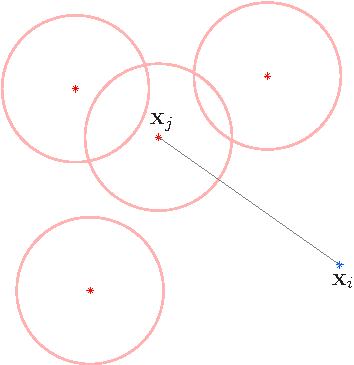
\includegraphics[width=6cm]{images/mog}}
%\subfigure[The projection $\AB$ applied to the whole data set $\mathcal{D}$.]{\label{fig:sub-sampling-2}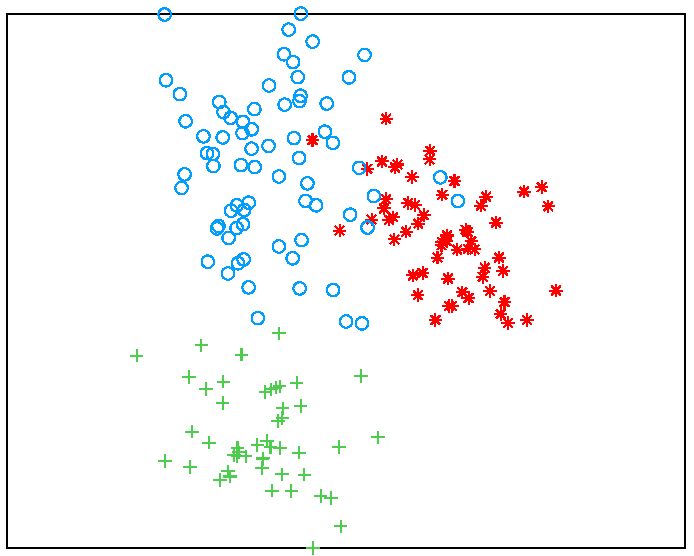
\includegraphics[width=0.48\textwidth]{images/sub-sample-2}}
  \caption{Formulating NCA as a class-conditional kernel density estimation framework.}
  \label{fig:kde}
\end{figure}

In this section we will present NCA into a class-conditional kernel density estimation framework. This interpretation will allow us to understand what are the assumptions behind NCA. Moreover, this also offers the possibility of altering the model in a suitable way that is efficient for computations. We will see this in the sections \ref{sec:approximate} and \ref{sec:exact-computations}. Similar ideas were previously presented by and , but the following were derived independently and they offer different insights. The following interpretation was inspired by the probabilistic $k$NN presented by \citet{barber2011}.

We start with the basic assumption that each class can be modelled by a mixture of Gaussians. For each of the $N_c$ data points in class $c$ we consider a Gaussian ``bump'' centred around it. From a generative perspective, we can view that each point $\xB_j$ can generate a point $\xB_i$ with a probability given by an isotropic normal distribution with variance $\sigma^2$:
\begin{align}
	p(\xB_i|\xB_j) &= \mathcal{N}(\xB_i|\xB_j, \sigma^2\mathrm{I}_D) \\
				   &= \frac{1}{(2\pi)^{D/2}}\exp \left\{-\frac{1}{2\sigma^2} (\xB_i - \xB_j)^\mathrm{T}(\xB_i - \xB_j)\right\}.
\end{align}

By changing the position of the points through a linear transformation $\AB$, the probability changes as follows:
\begin{align}
	p(\AB\xB_i|\AB\xB_j) \propto \exp \left\{-\frac{1}{2\sigma^2} (\xB_i - \xB_j)^\mathrm{T}\AB^\mathrm{T}\AB(\xB_i - \xB_j)\right\}.
\end{align}

We can note that this is similar to the $p_{ij}$ from NCA. Both $p(\AB\xB_i|\AB\xB_j)$ and $p_{ij}$ are directly proportional with the same quantity.

Using the mixture of Gaussians assumption, we have that the probability of a point of being generated by class $c$ is equal to the sum of all Gaussians in class $c$:
\begin{align}
	p(\xB_i|c) &= \frac{1}{N_c}\sum_{\xB_j \in c} p(\xB_i|\xB_j)\\
			   &= \frac{1}{N_c}\sum_{\xB_j \in c} \mathcal{N}(\xB_i|\xB_j, \mathrm{I}_D).
\end{align}

However, we are interested on the inverse probability, given a point $\xB_i$ what is the probability of $\xB_i$ belonging to class $c$. We can obtain an expression for $p(c|\xB_i)$ using Bayes' theorem:
\begin{align}
	p(c|\xB_i) = \frac{p(\xB_i|c)p(c)}{p(c|\xB_i)} = \frac{p(\xB_i|c)p(c)}{\sum_{c} p(\xB_i|c)p(c)}.
	\label{eq:nca-cc-kde-bayes}
\end{align}

Now if further consider the classes to be equal probable (which might a reasonable assumption if we have no a priori information) we arrive at result that resembles the expression of $p_i$ (see equation):
\begin{align}
%	&p(c|\xB_i) = \frac{p(\xB_i|c)}{\sum_{c} p(\xB_i|c)}\\
	p(c|\AB\xB_i) = \frac{
				\frac{1}{N_c}\sum_{\xB_j \in c}\exp\left\{-\frac{1}{2\sigma^2}(\xB_i - \xB_j)^\mathrm{T}\AB^\mathrm{T}\AB(\xB_i - \xB_j)\right\}
				}
				{
				\frac{1}{N_{c'}}\sum_{c'} \sum_{\xB_k \in c'}\exp\left\{-\frac{1}{2\sigma^2}(\xB_i - \xB_k)^\mathrm{T}\AB^\mathrm{T}\AB(\xB_i - \xB_k)\right\} 
				}
\end{align}

%In the numerator we have the sum of 
We are interested in predicting the correct class of the point $\xB_i$. So we try to find that linear transformation $\AB$ that maximises the class conditional probability of this point $p(c_i|\xB_i)$ to its true class $c_i$. 
\begin{align}
	f(\AB) = \sum_i p(c_i|\AB\xB_i).
	\label{eq:nca-cc-kde-obj}
\end{align}.

The gradient of the objective function is the following:
\begin{align}
	\frac{\partial f}{\partial \AB} = 
	  \sum_i \left\{ 
	  			\frac
	  			{
	  				\frac{\partial p(\AB\xB_i|c)}{\partial \AB}p(c)
	  			}
	  			{
	  				\sum_c p(\xB_i|c)p(c)
	  			}
	  			- \underbrace{\frac{
	  				p(\AB\xB_i|c)p(c)
	  			}{
	  				\sum_c p(\AB\xB_i|c)p(c)		
	  			}}_{p(c|\AB\xB_i)}
	  			\frac{
	  				\sum_c \frac{\partial p(\AB\xB_i|c)}{\partial \AB}p(c)
	  			}{
	  				\sum_c p(\AB\xB_i|c)p(c)
	  			}
	  	     \right \}.
	\label{eq:nca-cc-kde-grad}
\end{align}